
\chapter{Half a scheduling class}\label{chp:sched_idle}

% \hmng{transition??}
Within the Normal scheduling \textit{class}, Linux supports two different
scheduling \textit{policies}: \schednormal{} and \schedidle{}, where
\schednormal{} is the default. Under the hood, the scheduler for the Normal
class keeps the tasks of both policies on the same runqueue, and they are all
scheduled using the same algorithm. Thus, \schedidle{} is in principle not very
different from just being a low-weight process: From the scheduler's
perspective, \schedidle{} entities are just entities with a predefined low
weight (currently 3). There is, confusingly, also and Idle scheduling
\textit{class}, but that not accessible to userspace and exists solely to manage
the core's transition in and out of being actually idle (ie running nothing).

The main way that \schedidle{} entities are special-cased from \schednormal{}
entities is during wakeup: in 2019 a patch to Linux\cite{fixing-sched-idle-lwn}
added a check where, when a \schednormal{} entity becomes newly runnable, if the
core where the entity is waking up is already running something in
\schednormal{}, it will look for other cores that might be currently running a
\schedidle{} entity, and migrates the new entity there.

In doing so, Linux created a half scheduling class. In order to implement fully
invariant that no process of category B is ever running if a task of category A
is queued, that requires 1: checking if other cores are running a B task when an
A task wakes up on a core already running an A task, and 2: checking if another
core has a queued A task before running a B task.\ \schedidle{} does step 1, but
not step 2.

\schedidle{} is also promising because it was extended to have cgroup support
recently\cite{cgroup-idle-patch}: when set via the cpu.idle cgroup interface
file, the entire cgroup is counted as a \schedidle{} entity.

\begin{figure*}[t]
    \centering
    \begin{subfigure}[t]{0.48\textwidth}
        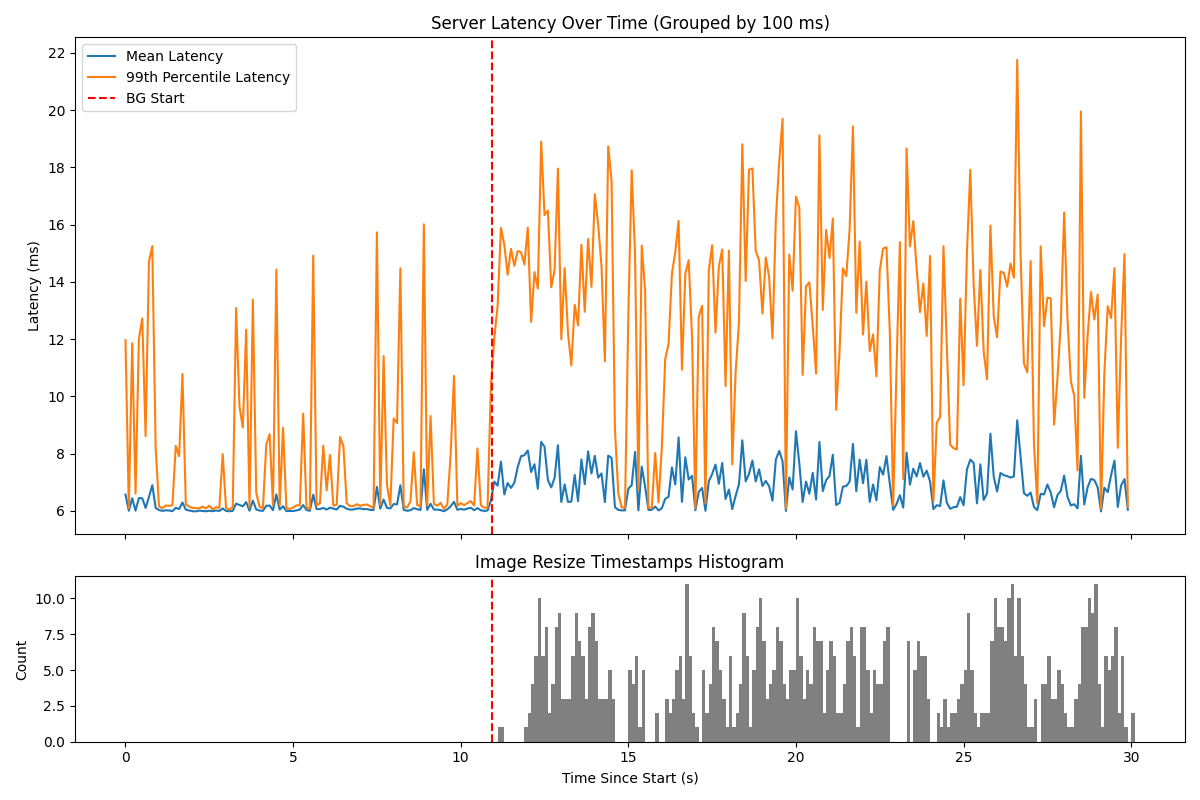
\includegraphics[width=\textwidth]{graphs/unedited-idle-low-two.png}
        \caption{Low load}\label{fig:unedited-idle-low-two}
    \end{subfigure}
    \hspace{\fill}
    \begin{subfigure}[t]{0.48\textwidth}
        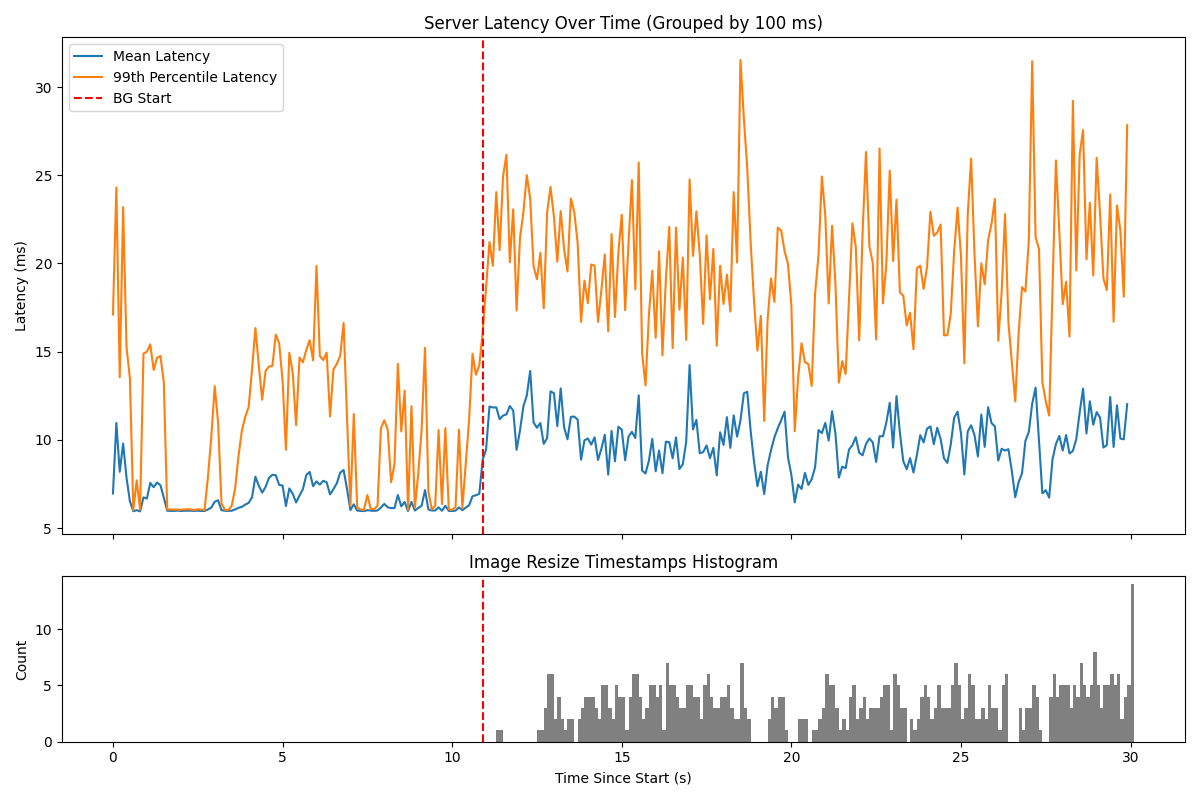
\includegraphics[width=\textwidth]{graphs/unedited-idle-high-two.png}
        \caption{High load}\label{fig:unedited-idle-high-two}
    \end{subfigure}
    \caption{using \schedidle{}}\label{fig:unedited-idle}
\end{figure*}

And indeed, we find that when we use cgroups' new cpu.idle interface feature,
the latency impact of the BE tasks decreases, although it does not entirely drop
to what we saw with the Fifo class. Figure~\ref{fig:unedited-idle} shows the
results, for the familiar settings of low and high load. The jump we see in the
mean latency has decreased from peaks as high as 13ms to around 7ms (even though
in principle they now have a higher weight).


